\documentclass[main]{subfiles}
\begin{document}

\section{関連研究}
\subsection{行動認識}
日本における少子高齢化の進行に伴い，医療・介護資源の不足は喫緊の課題である．
この解決策の一つとして，情報通信技術を活用して高齢者や障がい者の生活支援を行うAALが挙げられる．
AALは在宅での自立生活を促進することで，医療や介護で発生する労働時間や社会保障費などの社会的コストを抑制すると同時に，
被介護者の生活の質（Quality of Life; QoL）向上に寄与することを目指すものである\cite{blackman2016ambient}．\par

AALの要素技術である行動認識は，センサを用いて居住者の行動を認識し，異常行動の検知や健康状態の把握を行う．
従来の研究では，主にウェアラブルセンサ，カメラ，あるいはその他の環境設置型センサが用いられてきた．\par

ウェアラブルセンサは，対象者の状態を常時取得でき，転倒などの異常を即時に検知できる．
しかし，高齢者の認知機能低下に伴う装着忘れや充電等の管理不備のリスクが伴う．
加えて，常時機器を身につけることによる身体的な不快感や拘束感のみならず，被監視による心理的圧迫感が課題となることも考えられる\cite{guerra2023ambient}． \par

一方，カメラは情報量が豊富で具体的な行動認識が容易な上，身体への装着も不要である．
しかし，マイクと比較して導入コストが高くなりがちであり，プライバシーの観点から被介護者の心理的抵抗感が強い場合もある．
また，撮影範囲の死角や暗所における認識精度の低下も課題である\cite{guerra2023ambient,bouchabou2021survey}．\par

その他の非接触な手法として，家具や床に設置する圧力センサや，無線通信波の変動を利用して行動を検知する環境センサなどを利用する方法がある\cite{guerra2023ambient}．
これらは身体的負担がない点で優れるが，本稿ではこれらに加え，聴覚情報が持つ「環境音」や「発話」などの多面的な情報に着目する．\par

マイクは設置が容易でありながら，死角の影響を受けにくく，かつカメラよりもプライバシー受容性が高い．
特に，カメラの設置が倫理的に難しい浴室や洗面所においては，その有用性は高いと考えられる\cite{hyun2023sound}．
例えば，ヒートショックによる転倒や溺水が発生した際，流水音の継続や転倒時の衝撃音といった特定の音響イベントを捉えることで，
視覚的なプライバシーを侵害することなく異常を検知できる可能性がある．\par

しかし，実環境におけるマイクの運用には課題も残る．
換気扇の稼働音や生活雑音などの環境ノイズ，あるいは部屋の形状に起因する残響特性の違いが，
認識精度を低下させる要因となるためである\cite{mesaros2021sound}． 

本稿はマイクを含む複数のセンサを統合し，多様な文脈を考慮した柔軟な行動認識システムの構築を目的に，
その初期検討として，実環境におけるノイズなどの環境要因に対し，マイクによる行動認識精度を向上させる手法を検討する．\par

\subsection{音響イベント検出}
\label{section:sed}
他方， 音響信号から事象の種類と発生時刻を特定する音響イベント検出（SED）の研究が活発化している．
SEDは， 音響イベントのクラス識別および時間区間検出を同時に行う技術であり， 本稿では音による行動認識の手段としてこれを位置付ける．
本タスクではデータについて，10秒間の音声を「クリップ」，そのより細かな単位を「フレーム」と定義する．
これらはデータのラベルと対応する．「弱ラベル」はイベントの有無のみを示し，「強ラベル」はイベントの開始・終了時刻を含む．
これら二種類のデータを入力として受け取り，音から何が起きたか (イベント種別)とそれらの開始・終了時刻を予測する．これら予測は，ラベルと関連して弱予測，強予測と呼ぶ．\par
% 図解するかは後ほど判断

\begin{figure}[!htbp]
    \centering
    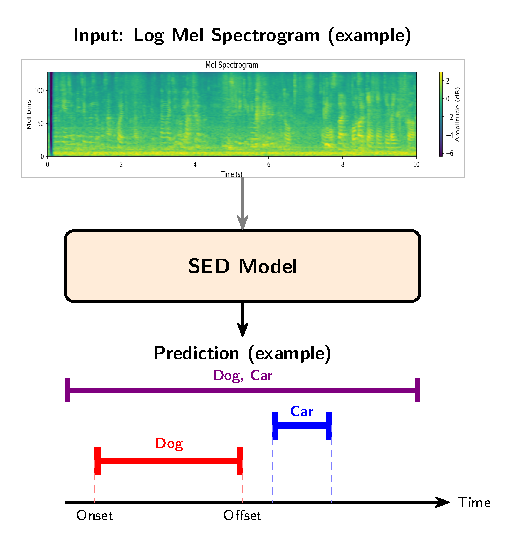
\includegraphics[width=80mm]{figures/sed.pdf}
    \caption{10秒の音声入力を対象とした予測の概略．全体におけるイベントの有無を判定する弱予測に対し，強予測ではイベントの区間（Onset/Offset）も算出する．注: 入力のスペクトログラムと予測結果はあくまで構造を説明するためのイメージであり，実際の対応はない．}
    % 図の説明をより詳細にする．
    \label{fig:sed}
\end{figure}
% \clearpage


\subsection{先行研究}
家庭内環境向けSEDのコンペディションとして， DCASEチャレンジが知られている． 
DCASE 2024 Task 4 (DCASE 2024)は， 大規模な未ラベルデータを用いた複数の事前学習済みモデルの活用が精度向上に寄与し， 上位成績を収めた\cite{schmid2024improving}．
 しかし， これらの手法はモデルの大規模化につながる可能性がある． 
 実環境への実装を想定した場合， モデルのパラメータ数増加は望ましくない． 
 本稿では， モデルサイズを維持しつつ精度を向上させることを目的に，半教師あり学習とドメイン汎化手法を改良及び統合する．\par

提案では，DCASE 2024の評価基準モデルを先行実装\footnote{\url{https://github.com/DCASE-REPO/DESED_task/tree/master/recipes/dcase2024_task4_baseline}}とする．
なお，本稿は基本的に先行実装の設定に準拠する\cite{cornell2024dcase}．\par
先行実装は半教師あり学習手法としてMean Teacher (MT) を用いる．図\ref{fig:meanteacher}にMTの概略を示す．
\begin{figure}[H]
    \centering
    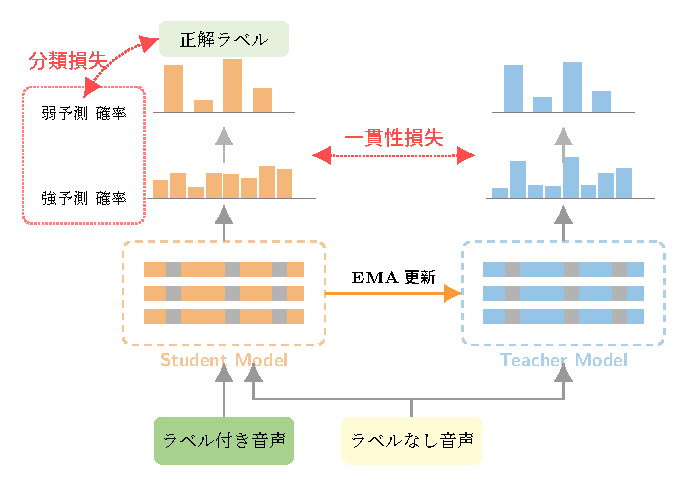
\includegraphics[width=0.9\columnwidth]{figures/mt_sed.pdf}
    \caption{MTの更新の概略．DESEDに対して適用する．Model内の灰色部は，モデルの一部にDropOutが適用され，ノイズ (摂動)として働くことを表す．}
    \label{fig:meanteacher}
\end{figure}


これは通常のモデルを「生徒」，生徒モデルの重みパラメータの移動指数平均 (Exponential Moving Average; EMA) を「教師」と定義し，入力にノイズが加わろうと教師と生徒の予測は同様という仮定の下，両予測の差を一貫性損失として扱う．この損失は平均二乗誤差で求められる．
MTでは，教師がラベルなしデータに対して行う予測を擬似的な目標値とし，生徒予測との一貫性を高めることで，ラベルなしデータを活用する\cite{tarvainen2017mean}．\par
MTに対してCMTは，教師予測に閾値を設け，信頼できる予測のみ学習に用いることで精度向上を図る\cite{xiao2023multi}．
 CMTは確率値が0.5より大きい予測のみ用いるが，閾値未満の確率値を持つ予測は損失に寄与せず，「イベントがない」ことの学習が難しい．
 当環境で検証したところ，CMTはMTに比べてイベントの分類予測精度を向上したが，イベントの開始や終了時刻の予測精度（時間的な精度）は低下した．
 なお，CMT及びその検証を行った論文ではイベント分類及び時間境界の精度の向上が報告されていた\cite{11036061}．\par
本研究での提案として，確率値0.7以上の予測を正例，0.3以下の予測を負例とし，両方を学習する．CMTに比べ，あまり自信のない確率値0.5付近の予測を使わず，より安定した精度が得られると共に，フレーム単位での「イベントがない」ことを学習することで，時間的精度の向上が期待される．\par

次に，ドメイン汎化について述べる．ここでドメインとは，同一のクラスラベルであっても，データが観測された環境や条件によって生じる特徴分布の違いを指す．
例えば，画像認識では実写とイラストが異なるドメインとして扱われる．同様に，録音環境や背景雑音の違いにより，種類の同じ音響イベントでも周波数などの特徴が異なる．
モデルがこうした環境依存の情報に過剰適合することを防ぎ，未知の環境でもロバストな推論を可能にすることがドメイン汎化の目的である．\par

MixStyle\cite{zhou2021domain}はドメイン汎化に有効なデータ拡張手法の一つである．
先行研究\cite{xiao2024fmsg}において周波数領域の注意機構との統合が示唆されているが，その具体的なアーキテクチャは詳述されていない．
そこで本稿では，より軽量な畳み込みニューラルネットワーク (Convolutional Neural Network; CNN) での統合を提案する． 
\end{document}